\section{Introduction}

High-fidelity simulations of high-dimensional dynamical systems
can be expensive when repeated predictions are required across many parameter settings. Reduced-order models (ROMs) provide a cost-effective surrogate by representing the physical state with a small number of state variables. The problem becomes more challenging when changing a parameter also changes the type of regimes. In incompressible flows, for example, varying the Reynolds number can lead from relaxation toward a steady state to oscillatory growth and sustained periodic motion. A useful predictive model must capture these regimes while evolving autonomously.



Such regime variation introduces two closely related challenges for ROMs. The first concerns representation: spatial structures that are important in one regime may differ from those required in another, making a single representation less effective. The second is dynamical: the reduced evolution law must accommodate qualitatively different behaviors, including stable relaxation, instability growth, and nonlinear periodic oscillations. Increasing model capacity alone cannot compensate for an inadequate reduced representation, while improving the representation does not by itself guarantee accurate autonomous rollout. These observations motivate adapting the local representation and the local dynamics separately, while providing a consistent way to assemble their predictions.




Projection-based ROMs provide an explicit reduced representation and reduced dynamics, commonly through proper orthogonal decomposition (POD) and Galerkin projection \citep{sirovich1987,berkooz1993,benner2015}. However,projection-based ROMs are inherently affected by truncation, which neglects the influence of discarded modes on the retained coordinates, leading to closure errors that degrade long-horizon prediction.\citep{amsallem2012}. Data-driven ROMs offer greater flexibility in approximating nonlinear dynamics, but low one-step error does not guarantee accurate autonomous rollouts, and they often lack physical interpretability\citep{duraisamy2019,brunton2020}. Hybrid ROMs combine projection-based ROMs with learned corrections or learned reduced representations, retaining physical structure while increasing approximation flexibility
\citep{dar2023,lee2020,fresca2022,geelen2023}. These developments improve the modeling of reduced dynamics, but they do not by themselves resolve the representational difficulty that arises when qualitatively different regimes must be described over a broad parameter range.





A complementary strategy localizes the reduced representation, using multiple subspaces, clusters, or manifolds for different portions of the solution set \citep{kaiser2014,li2021cluster,diaz2024}. These directions address complementary aspects of the broad-parameter problem: hybrid modeling improves the fidelity of the reduced dynamics, whereas localization adapts the reduced representation to regime-dependent structures. Localization, however, creates a new assembly problem.  Independently constructed local ROMs generally have different reduced state variables and  operators, so their reduced coordinates are chart-specific. Direct interpolation or averaging in reduced-coordinate space therefore has no natural cross-chart interpretation. Mixture-of-experts (MoE) architectures provide a natural framework for conditional specialization \citep{jacobs1991,jordan1994,shazeer2017,fedus2022}, but standard MoE formulations typically route specialized predictors within a shared representation or common feature space. Here, in contrast, the experts are complete local ROMs whose coordinates are not shared. The problem is therefore not only routing among local ROMs, but also assembling or fusing their outputs across representations. This makes the problem hierarchical: one must adapt the reduced dynamics within each local representation and, separately, route to and fuse complete local ROMs across representations. This raises a distinct question that standard within-representation MoE routing does not address: how can independently constructed local dynamical models be routed and assembled without forcing them into a common latent coordinate system?


To address this gap, we introduce the Regime-Adaptive Localized Mixture-of-Experts Reduced-Order Model (RAL-MoE-ROM), a two-level hierarchical framework that separates regime-local reduced dynamics from cross-regime routing and fusion. The parameter domain is covered by prescribed, overlapping regime-local regions, each equipped with an independent  autonomous specialist. At the first level, each specialist, use an explicit projected-based ROM  and augments it with sparsely  structured MOEs which trained trained through  multi-step autonomous rollouts. Rather than using conventional MLP-only experts, each activated expert decomposes its output into three additive components: a nonlinear neural branch, together with explicit linear and low-rank quadratic branches derived from the projection-based. At the second level, a parameter-conditioned outer router produces window-level routing weights over the local specialists, while a fixed applicability mask determines whether inference uses one specialist or a pair of adjacent specialists. When two specialists are selected, a learned fusion gate combines their reconstructed physical fields conditioned on the initial physical history. The overall architecture is illustrated in Figure~\ref{fig:ral_overview}, highlighting the regime-local specialists and the cross-regime routing and fusion mechanism.




Our main contributions are as follows:
\begin{itemize}

\item \textbf{Structured regime-local specialists for autonomous reduced dynamics.} Each specialist combines a physics-based ROM with a structured sparse MoE closure and is trained under closed-loop multi-step rollouts.

\item \textbf{Cross-regime routing and fusion.}
An outer router selects a specialist or a pair of neighboring specialists. When two specialists are selected, a learned gate uses the initial physical history to combine their reconstructed fields.

\item \textbf{Multi-regime evaluation.}
We evaluate the framework on  incompressible-flow benchmarks spanning steady, Hopf-onset, and periodic regimes. The experiments assess autonomous specialist rollouts, cross-regime routing and fusion in regime overlaps, and the main local architectural choices, providing complementary evidence for the proposed local modeling and assembly strategy.

\end{itemize}




\par
\begin{figure}[t]
    \centering
    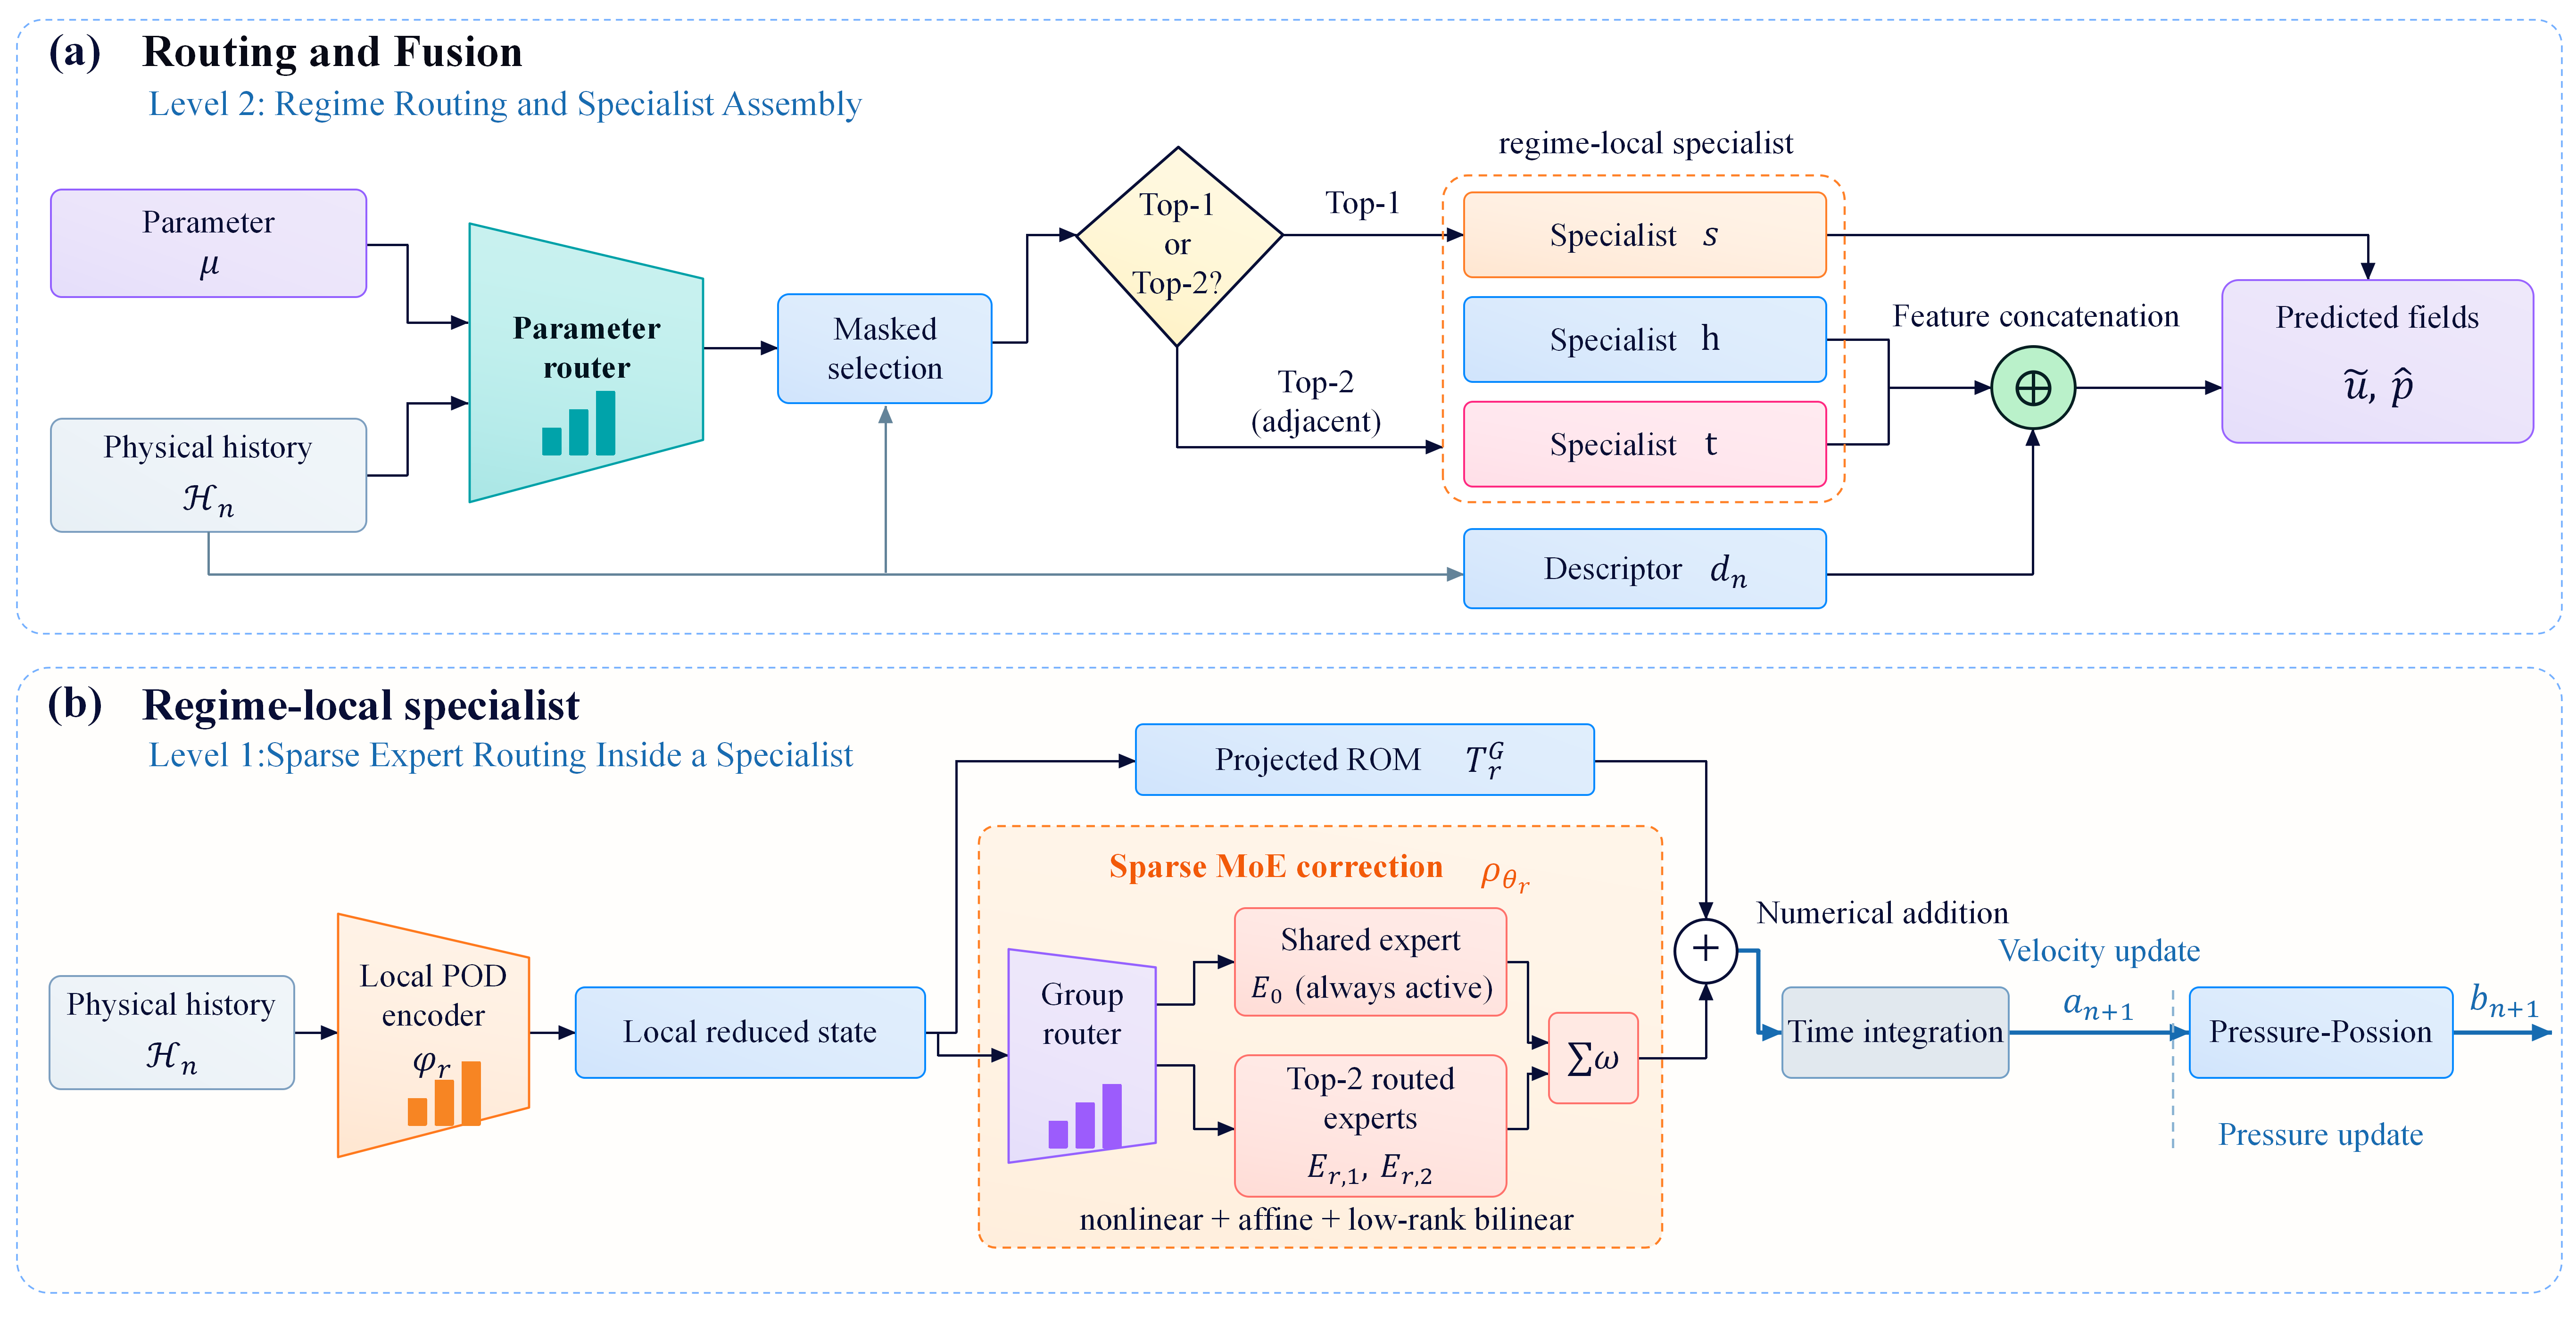
\includegraphics[width=\linewidth]{figures/flowchat.png}
\caption{
Overview of RAL-MoE-ROM.
(a) A parameter-only outer router provides trajectory-level preferences over regime-local specialists, while an applicability mask restricts inference to a single specialist or an adjacent pair. When an adjacent pair is used, a history-conditioned
gate combines only their reconstructed physical fields.
(b) Each regime-local specialist augments a projected ROMs  with a structured sparse MoE correction.
}
    \label{fig:ral_overview}
\end{figure}
\par


